\documentclass[paper=a4, fontsize=10pt]{jlreq}

\usepackage{amsmath, amssymb}
\usepackage{enumerate}
\usepackage{tikz}
\usepackage{graphicx}
\usepackage{listings, xcolor}

\lstset{
  basicstyle = {\ttfamily},
  frame = {tbrl},
  breaklines = true,
  numbers = left,
  showspaces = false,
  showstringspaces = false,
  showtabs = false,
  keywordstyle = \color{blue},
  commentstyle = {\color[HTML]{1AB91A}},
  identifierstyle = \color{black},
  stringstyle = \color{brown},
  captionpos = t
}

% C#用の言語定義を追加
\lstdefinelanguage{CSharp}{
  keywords={class, public, private, void, using, namespace, if, return, new, float, Vector3, Rigidbody},
  sensitive=true,
  morecomment=[l]{//},
  morestring=[b]"
}

\title{情報学群実験第4 実験レポート}
\author{学籍番号 1280391 \\ 細川 夏風}
\date{\today}

\begin{document}

\maketitle

\section{目的}
近年の急速な情報技術の発展により，現実世界以上に活動の幅を広げることが増えた．その最たる例として\texttt{Virtual Reality(VR)}が挙げられる．\texttt{VR}には制限が極端に少ないように感じる．しかし，その実は多くの制限が存在する．それは多くがヒト自体の肉体的制限や特性に依るものであることが多い．今実験では，そのヒトの制限や特性を理解し，より没入感のある\texttt{VR}体験を提供するための検証を行う．

\section{方法}
本実験は，視覚探索課題を行う心理物理実験の実施と，得られたデータに対する回帰分析および統計的仮説検定の$2$つの段階に分けて実施した．

次実験の\texttt{VR}ゲーム作成では，\texttt{Unity}を用いた$3$\texttt{D}ゲームの開発と，\texttt{Meta Quest} $3$\texttt{S}および\texttt{Meta XR SDK}を用いたバーチャルリアリティ（\texttt{VR}）環境への対応という$2$つの段階で実施した．

\subsection{心理物理実験の実施（視覚探索課題）}
実験プログラムは\texttt{Python}および\texttt{Psychopy}を用いて作成された\texttt{visualsearch.py}を使用した[付録\ref{src:visualsearch}]．
実験参加者は，ディスプレイまでの観察距離を一定に保ち，画面上に提示される妨害刺激の中に目標刺激が存在するか否かを可能な限り早く，かつ正確に判断する課題を行った．
刺激の条件として，目標刺激には「丸」および「丸＋棒」の$2$種類を用いた．目標刺激が「丸」のときの妨害刺激は「丸＋棒」であり，目標刺激が「丸＋棒」のときの妨害刺激は「丸」とした．
提示される刺激の総数（セットサイズ）は$4$，$8$，$16$個のいずれかであり，目標刺激が$1$つ存在する試行と，目標刺激がなく妨害刺激のみの試行がランダムな順序で提示された．
参加者は，目標刺激がある場合は「\texttt{J}」キーを，ない場合は「\texttt{F}」キーを押して回答した．
実験は$12$試行の練習試行を行った後，$240$試行の本実験を実施した．なお，課題の処理自体にかかる時間以外の要因を排除するため，反応に$5$秒以上かかった時間オーバーの試行および不正解だった試行のデータは分析から除外した．

\subsection{データ分析および統計的仮説検定}
心理物理実験で得られた各自の反応時間データについて，目標刺激の種類，有無，およびセットサイズごとに平均値を算出した後，複数人数分のデータを取りまとめた．
まとめたデータに基づき，各条件における反応時間の平均値，不偏分散，標準偏差，および標準誤差を算出した．
次に，横軸をセットサイズ，縦軸を反応時間とする散布図を作成し，各条件の平均値のプロットと標準誤差を示す誤差線を付加した．
得られたプロットに対して単回帰分析を行い，セットサイズに対する反応時間の回帰直線の傾きを算出した．
最後に，目標刺激が存在する条件において，目標刺激が「丸」のときと「丸＋棒」のときで回帰直線の傾きの平均値に統計的な有意差があるかを確認するため，対応のある$t$検定を用いた統計的仮説検定を実施した．

\begin{figure}[htbp]
  % 1つ目の画像（全体の45%の幅を割り当て）
  \begin{minipage}[b]{0.45\linewidth}
    \centering
    
\includegraphics[width=0.8\linewidth]{circle.png}
    \caption{丸の目標刺激}
    \label{fig:circle}
  \end{minipage}
  % 中央に少し空白を空ける
  \hfill
  % 2つ目の画像（全体の45%の幅を割り当て）
  \begin{minipage}[b]{0.45\linewidth}
    \centering
    
\includegraphics[width=0.8\linewidth]{circle_bar.png}
    \caption{丸＋棒の目標刺激}
    \label{fig:circle_bar}
  \end{minipage}
\end{figure}

\subsection{VR実験環境および使用機器}
本実験で使用した主な環境および機器・ソフトウェアは以下の通りである．

\begin{itemize}
  \item \textbf{心理物理実験（視覚探索課題）}
  \begin{itemize}
    \item \texttt{PC}
    \item \texttt{Python}および\texttt{Psychopy}（バージョン$2026.1.3$）
  \end{itemize}
  \item \textbf{$3$\texttt{D}ゲームおよび\texttt{VR}コンテンツの開発}
  \begin{itemize}
    \item \texttt{VR}対応ゲーミング\texttt{PC}
    \item \texttt{Meta Quest} $3$\texttt{S}ヘッドセット
    \item \texttt{Meta Link}ケーブル（または\texttt{USB-C}ケーブル）
    \item \texttt{Unity} $6$（エディターバージョン$6000.1.11$\texttt{f}$1$）
    \item \texttt{Meta Horizon Link}アプリ
    \item \texttt{Meta XR All-in-One SDK}
    \item \texttt{Visual Studio}（\texttt{C\#}スクリプト作成・編集・デバッグ用）
  \end{itemize}
\end{itemize}

\subsection{$3$\texttt{D}ゲームの基礎開発}
\texttt{Unity} $6$を用いて，「ボールを転がしてコインを集める」$3$\texttt{D}ゲームの開発を行った．
まず，\texttt{Cube}を利用して床と壁を作成し，\texttt{Sphere}を用いてプレイヤーとなるボールを作成した．プレイヤーには\texttt{Rigidbody}コンポーネントを追加し，物理演算を適用した．
次に，\texttt{C\#}スクリプトを作成し，\texttt{FixedUpdate}関数内で\texttt{Rigidbody.AddForce}を用いることで，キーボード入力によるプレイヤーの移動を実装した[付録\ref{src:MovePlayer}]．また，プレイヤーに追従してカメラが移動するスクリプト[付録\ref{src:FollowPlayer}]や，\texttt{Cylinder}で作成したコインを回転させるスクリプト[付録\ref{src:RotateCoin}]を作成した．
さらに，プレイヤーがコインのタグに触れた際にコインを非表示にし，\texttt{TextMeshPro}を用いて画面上にスコアと経過時間（タイマー）を表示する機能を実装した．最後に，作成したシーンをテンプレートとして保存し，複数のステージを作成した．全コイン獲得後に特定のキーを入力することで，次のステージへ遷移する処理も実装した．

\subsection{\texttt{VR}環境への対応とインタラクションの実装}
作成した$3$\texttt{D}ゲームを\texttt{VR}環境で体験できるようにするため，\texttt{Meta Quest} $3$\texttt{S}ヘッドセットと\texttt{PC}を\texttt{Quest Link}を用いて接続した．
\texttt{Unity}プロジェクト内で\texttt{XR Plugin Management}を有効にし，\texttt{Meta XR All-in-One SDK}を導入した．
その後，\texttt{Building Blocks}機能から\texttt{Camera Rig}をシーンに追加し，\texttt{VR}空間での視点を構築した．また，\texttt{Canvas}のレンダーモードを\texttt{World Space}に変更し，\texttt{VR}空間内にスコア等の\texttt{UI}が表示されるように調整した．
さらに，\texttt{Grab Interaction}などの機能を導入し，キーボードではなくハンドトラッキングを用いてゲーム内のボードを手でつかんで傾けることで，ボールを転がしてコインを集められるように操作方法を変更した．

\subsection{ビリヤードゲームの作成}
最終的に自班ではビリヤードゲームの作成を行った．プレイヤーは，開始時に眼の前にある棒を手で掴みゲームを始める．プレイヤーはビリヤード台に配置されている$6$つの番号つきボールを棒で転がした白いボールですべて穴に行けることとによってゲームが終了する．ゲーム終了時は，スコアと経過時間が表示される．このとき，穴の下にコインを配置し，ボールが穴に入るとコインが獲得できる仕組みになっている．ゲーム中はプレイヤーの持つコントローラーの左スティックを傾けることで移動が可能になっている．このゲームはビリヤードゲームであるがルールに関しては簡略化されており，ボールを穴に入れる順番は問わない．また，この時使用した\texttt{Asset}は\texttt{Unity Asset Store}で入手したものを付録に示しておく[付録\ref{sec:asset}]．

\section{結果}

\subsection{統計分析}
視覚探索課題における反応時間について，条件ごとおよびセットサイズごとの平均値を算出した結果を表\ref{tab:result_mean}に示す．

\begin{table}[htbp]
  \centering
  \caption{各条件における反応時間の平均値（\texttt{ms}）}
  \label{tab:result_mean}
  \begin{tabular}{|c|c||c|c|c|}
    \hline
    目標刺激 & 目標刺激の有無 & セットサイズ$4$ & セットサイズ$8$ & セットサイズ$16$ \\ \hline \hline
    丸 & あり & $773$ & $886$ & $950$ \\ \hline
    丸 & なし & $791$ & $931$ & $1046$ \\ \hline
    丸＋棒 & あり & $684$ & $672$ & $682$ \\ \hline
    丸＋棒 & なし & $702$ & $700$ & $731$ \\ \hline
  \end{tabular}
\end{table}

\begin{figure}[htbp]
  \centering
  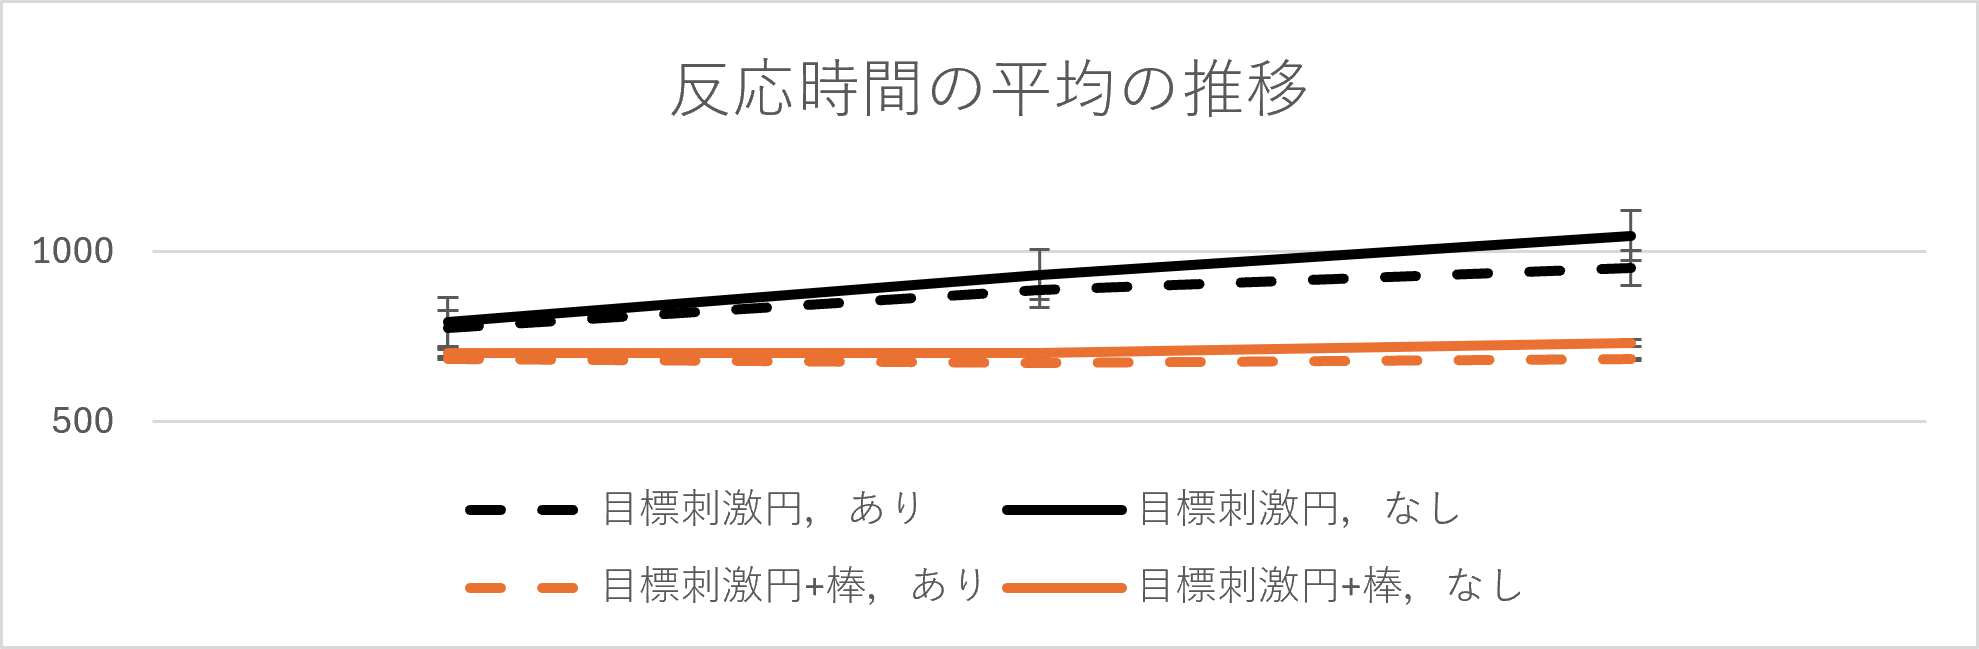
\includegraphics[width=0.9\linewidth]{画像3.png}
  \caption{各条件におけるセットサイズと反応時間の関係}
  \label{fig:result_graph}
\end{figure}

\begin{table}[htbp]
  \centering
  \caption{目標刺激あり条件における回帰直線の傾きの$t$検定結果}
  \label{tab:t_test_result}
  \begin{tabular}{|c|c|}
    \hline
    $t$値 & $p$値 \\ \hline
    $3.02$ & $0.0165$ \\ \hline
  \end{tabular}
\end{table}

また，目標刺激が存在する条件（あり条件）において，目標刺激が「丸」のときと「丸＋棒」のときで回帰直線の傾きの平均値に有意な差があるかを確認するため，対応のある$t$検定を行った．
その結果，$t$値は約$3.02$，$p$値は約$0.0165$となり，有意水準$5$\%において統計的に有意な差が認められた．

\subsection{VRゲームの作成}
\texttt{Unity}および\texttt{Meta Quest} $3$\texttt{S}を用いた\texttt{VR}コンテンツ開発の結果として，ビリヤードゲームを作成した．
本コンテンツは，初期に開発した「ボールを転がしてコインを集める」ゲームの知見を発展させたものであり，\texttt{VR}空間内にビリヤード台や複数の的球，キューなどを配置して構築した．また，タイマー機能やスコア機能も実装している．\texttt{Meta XR SDK}の機能を活用することで，プレイヤーは\texttt{VR}環境においてハンドトラッキング等のインタラクションを用いて実際のビリヤードのような操作を体験することができる．
作成したビリヤードゲームの\texttt{Unity}での開発画面を図\ref{fig:billiard2}に，\texttt{VR}環境でのプレイ画面を図\ref{fig:billiard}に示す．

\begin{figure}[htbp]
  \begin{minipage}[b]{0.45\linewidth}
    \centering
    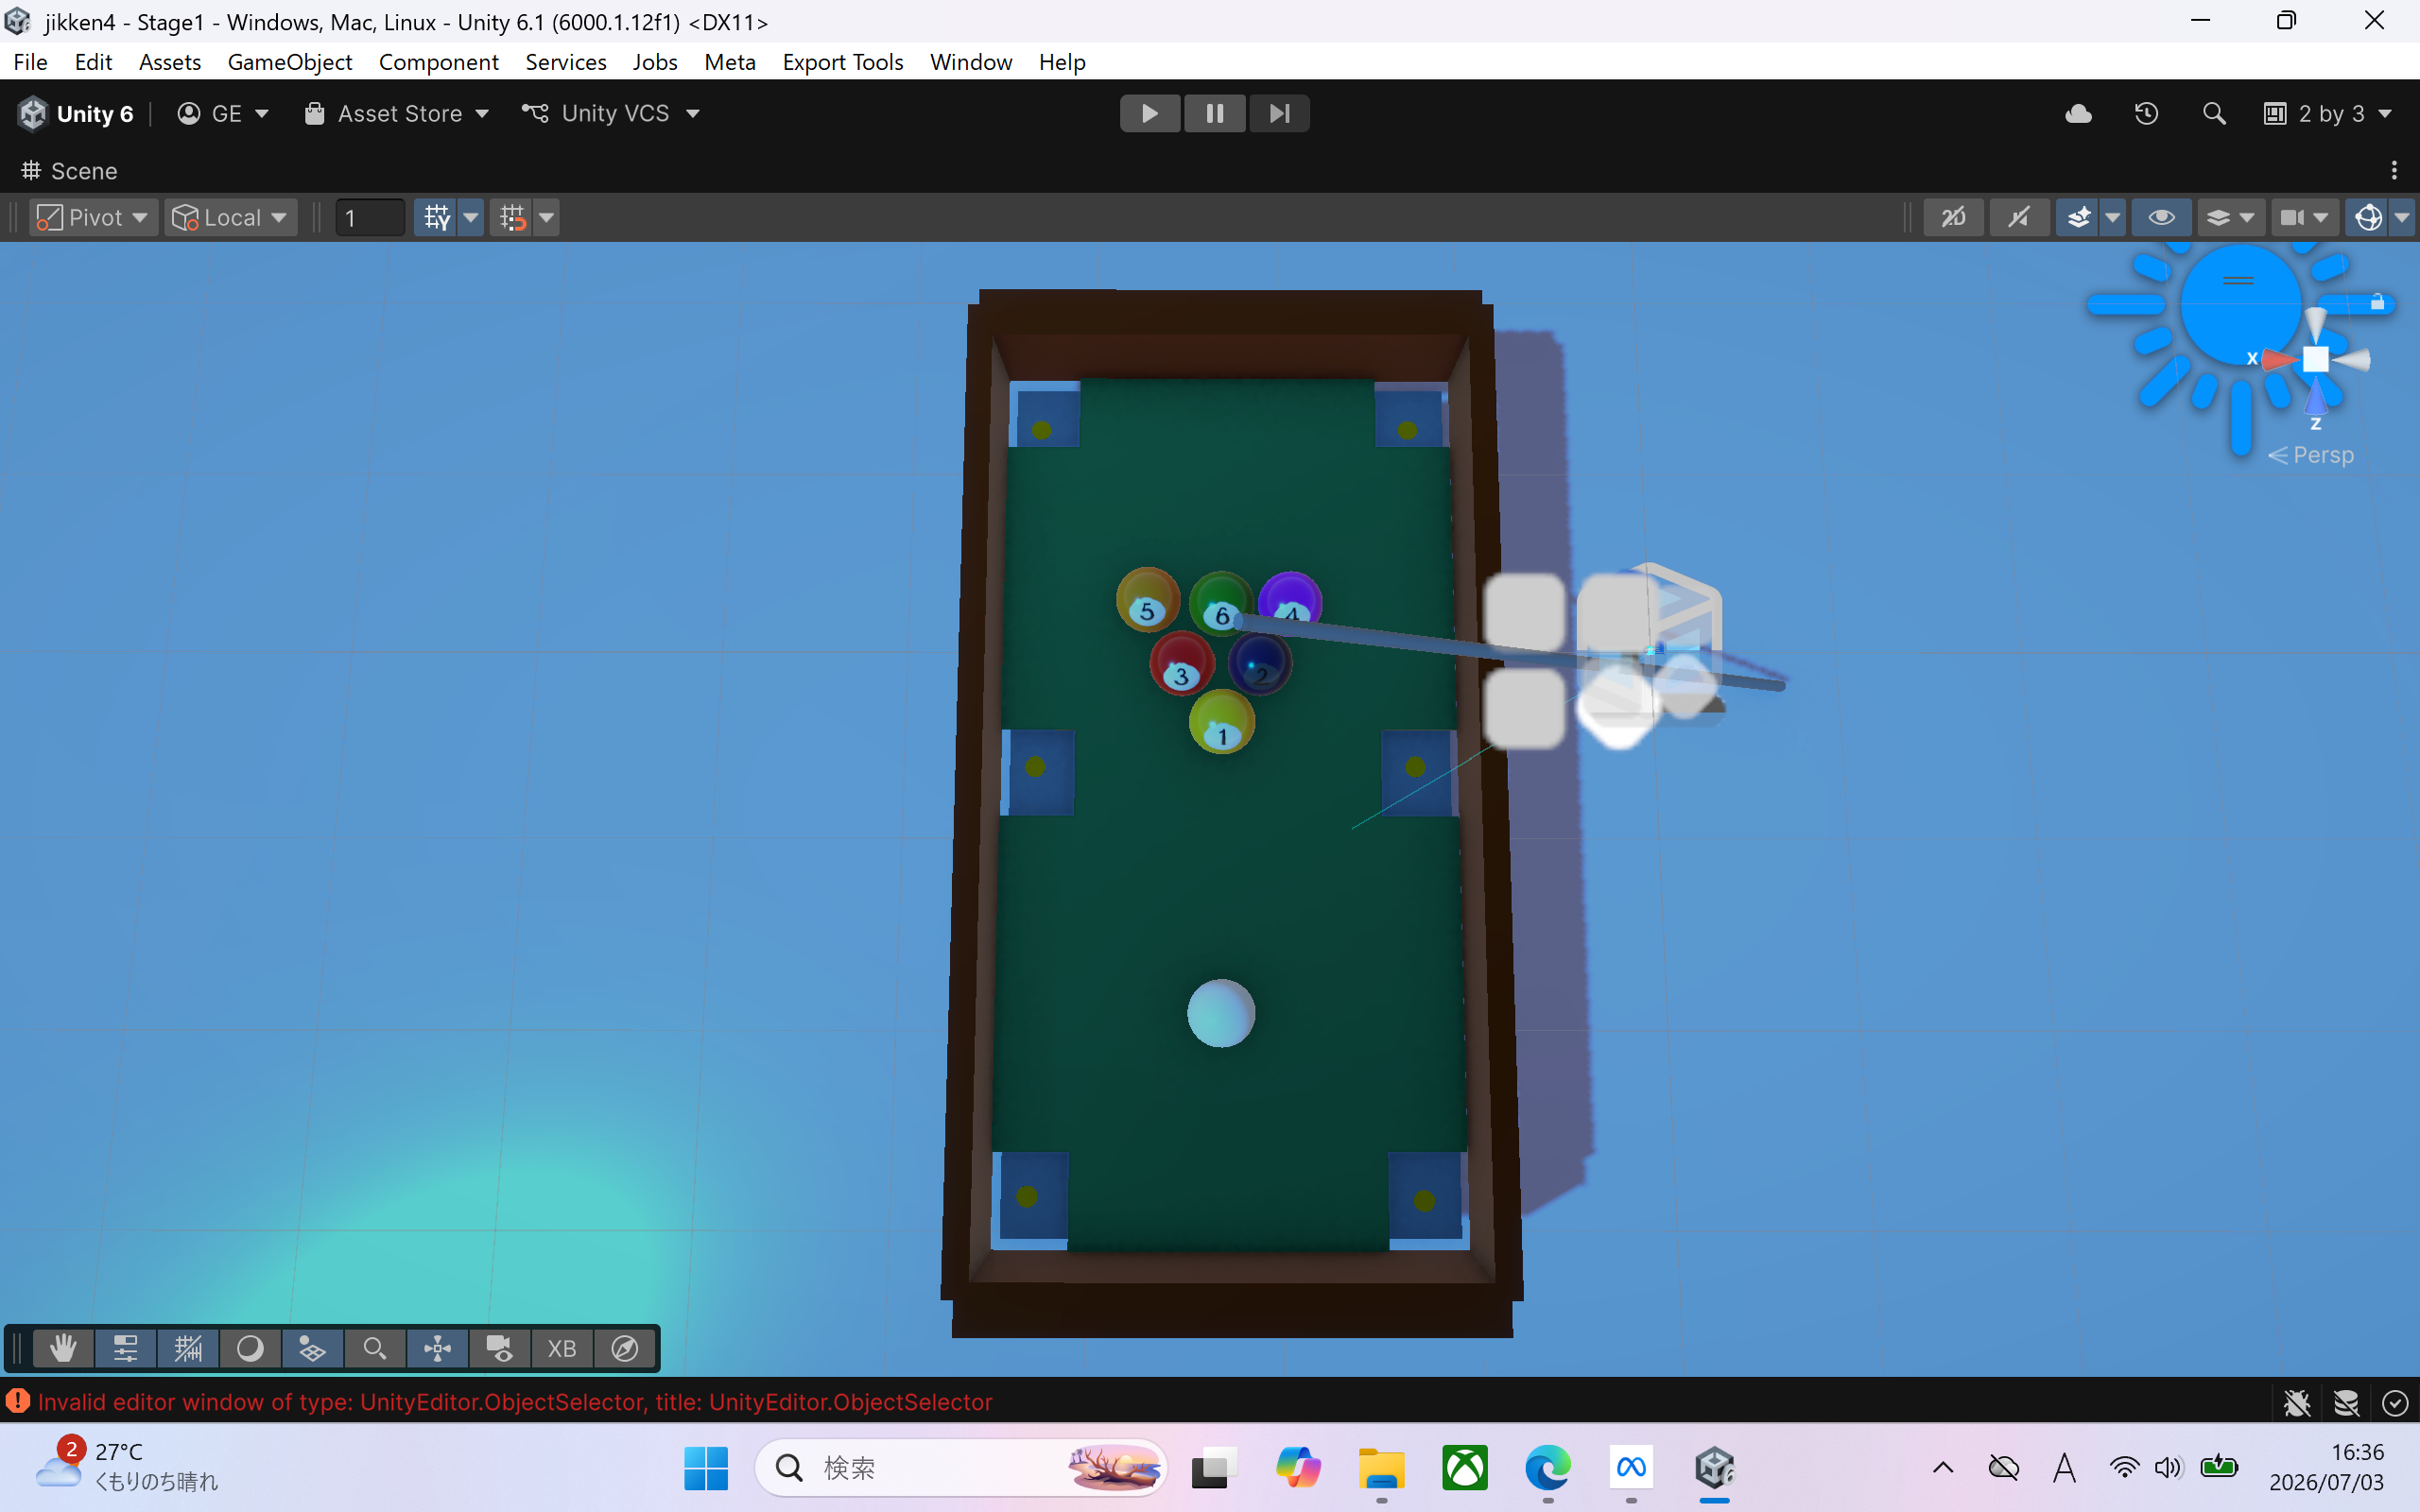
\includegraphics[width=\linewidth]{ビリアード2.png}
    \caption{\texttt{Unity}でのゲーム開発画面}
    \label{fig:billiard2}
  \end{minipage}
  \hfill
  \begin{minipage}[b]{0.45\linewidth}
    \centering
    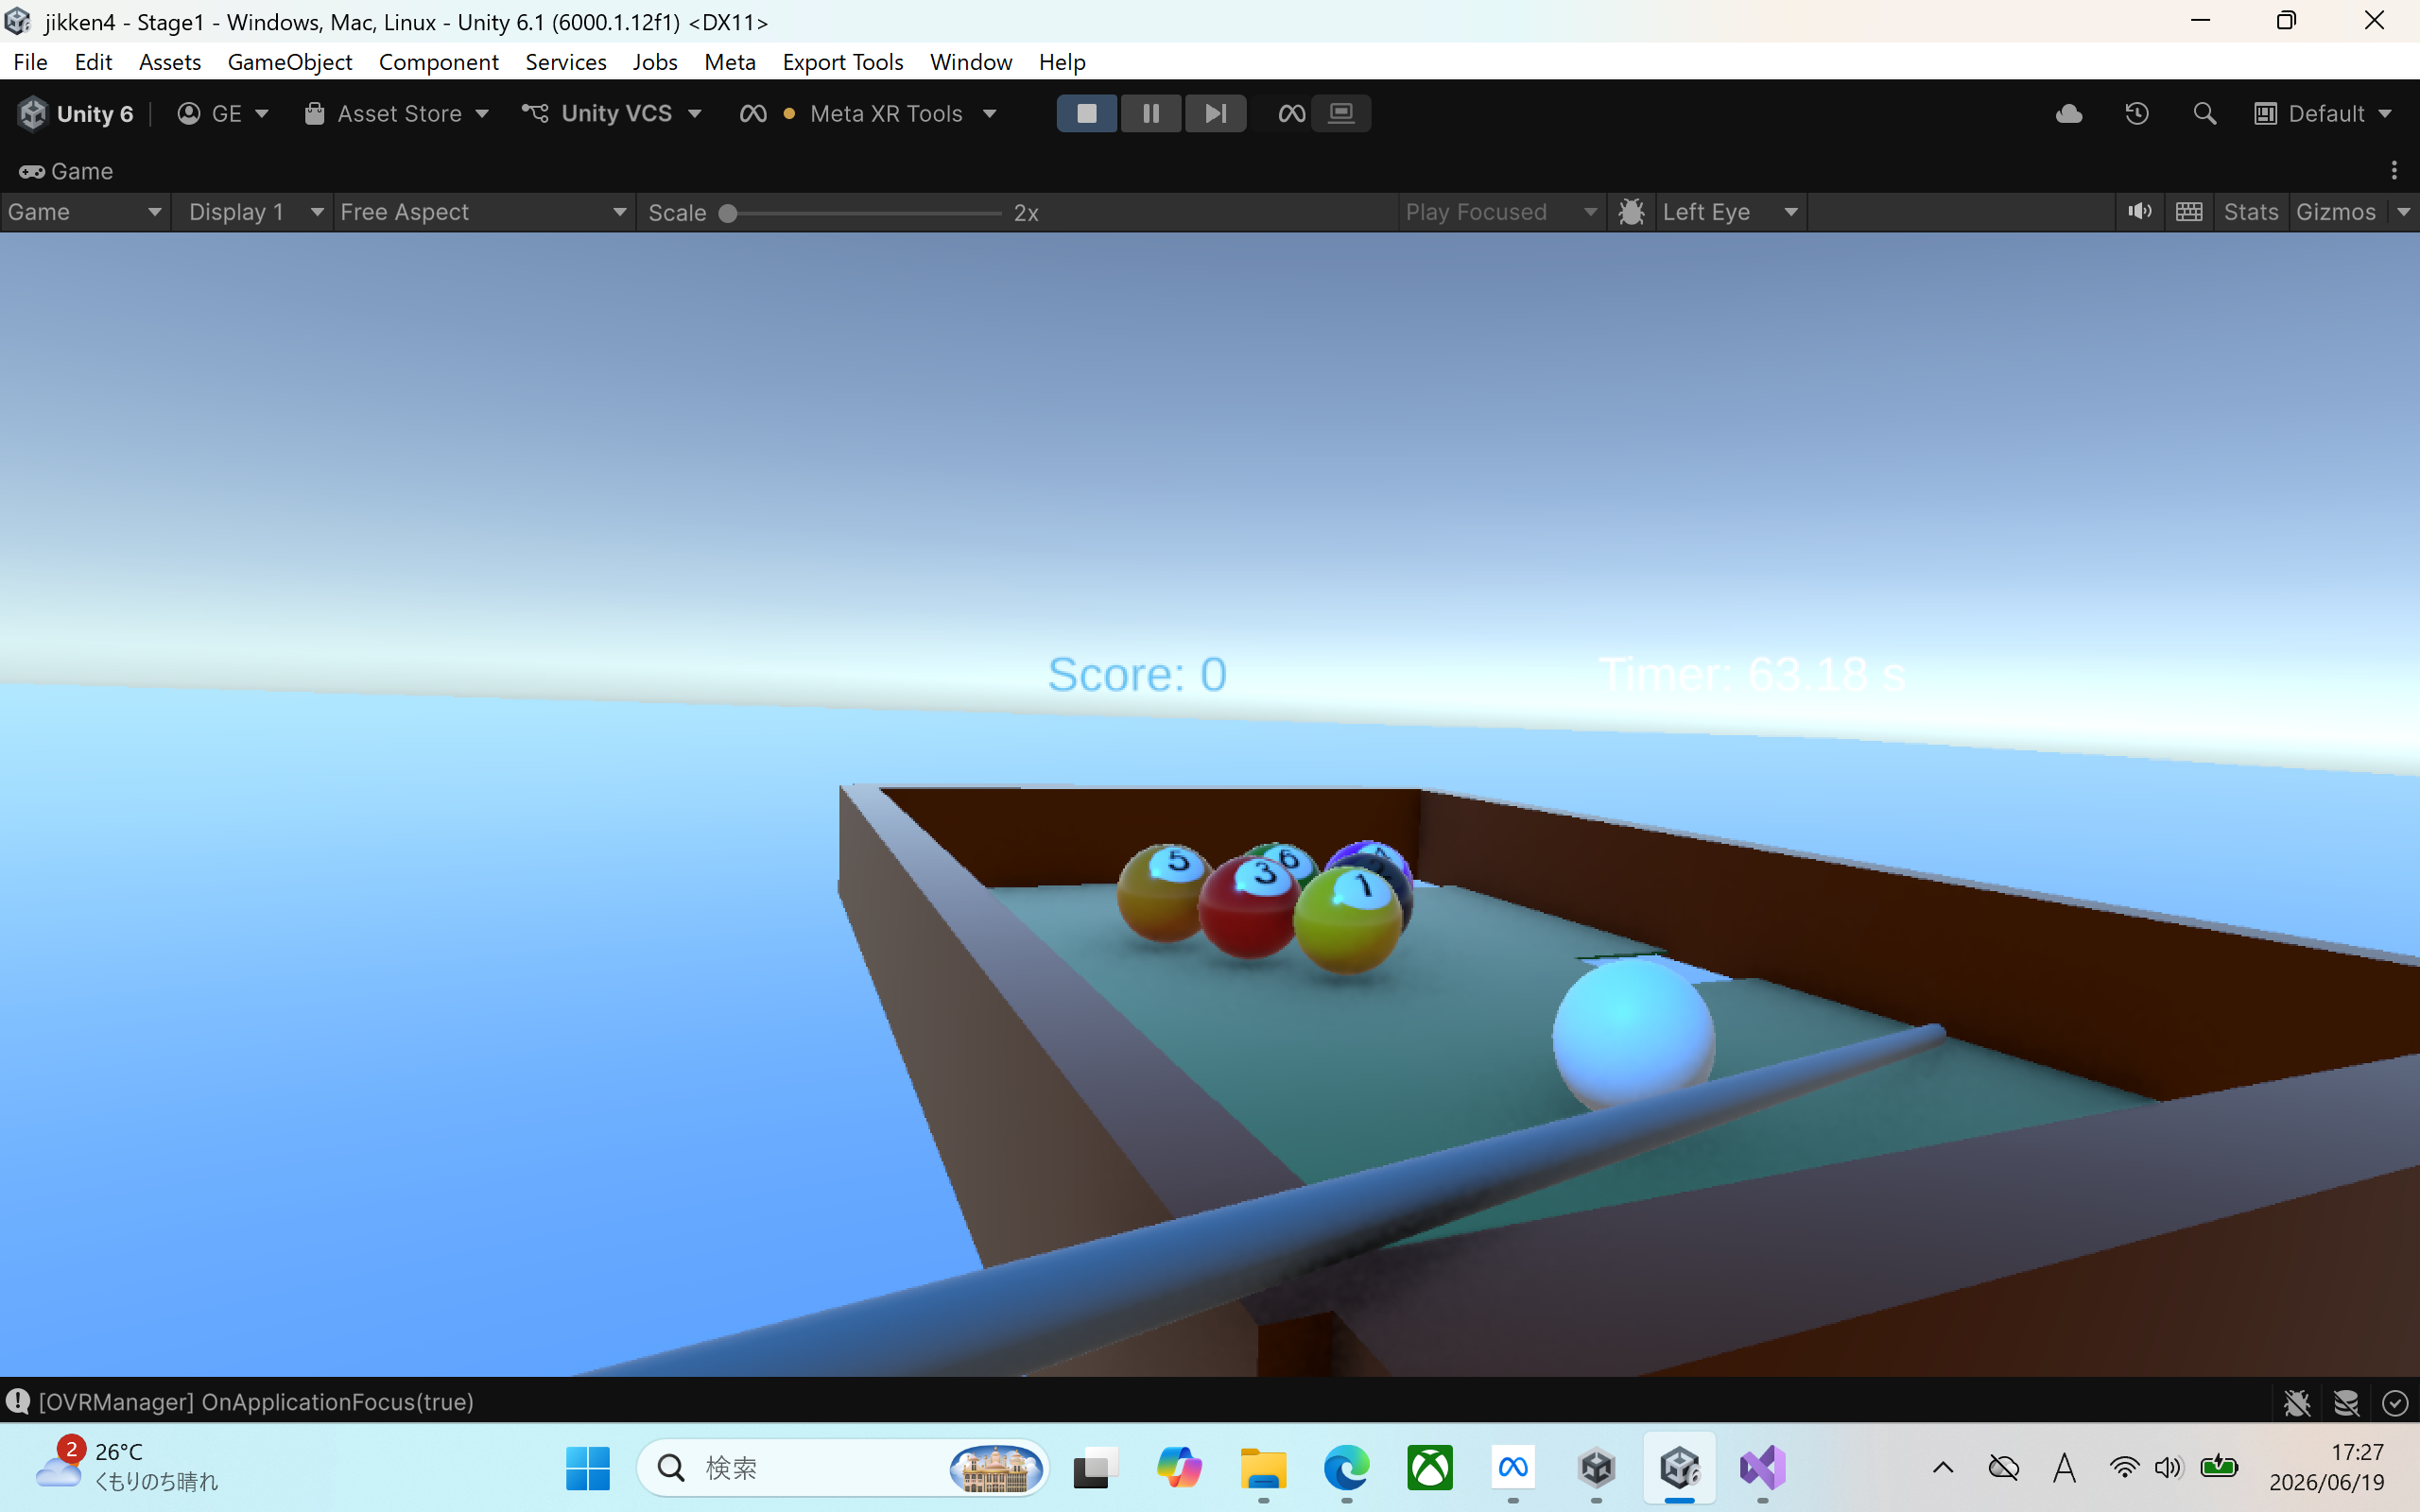
\includegraphics[width=\linewidth]{billiard.png}
    \caption{\texttt{VR}環境でのプレイ画面}
    \label{fig:billiard}
  \end{minipage}
\end{figure}

\section{考察}

\subsection{視覚探索課題における反応時間の傾向}
本実験結果から，目標刺激の条件によってセットサイズに対する反応時間の増加率に顕著な違いが見られた．目標刺激が「丸＋棒」の条件では，セットサイズが増加しても反応時間はほぼ一定であった．一方，目標刺激が「丸」の条件では，セットサイズが増加するのに比例して反応時間が顕著に増加した．また，対応のある$t$検定の結果からも，$2$条件の回帰直線の傾きには有意な差があることが示された．加えて，目標刺激ありの条件に対して，なしの条件の方が全体的に反応時間が長くなる傾向も確認された．

\subsection{特徴統合理論と探索非対称性による解釈}
これらの結果は，Treismanらが提唱した特徴統合理論\cite{bsd_attention}および視覚探索の非対称性の観点から説明できると考えられる．
妨害刺激である「丸」の中に，目標刺激「丸＋棒」が存在する場合，「棒」という初期的な視覚特徴が前注意的段階で素早く検出され，ポップアウト現象が生じる．この場合，視覚情報は並列的に処理されるため，セットサイズに依存せず短い反応時間で目標を検出できたと推測できる．

これに対し，妨害刺激である「丸＋棒」の中に，目標刺激「丸」が存在する場合，目標刺激は「棒がない」という特徴の欠如によって定義される．特徴統合理論によれば，特徴の欠如はポップアウトを引き起こさないため，注意を各刺激に順番に向ける直列的な処理を強いられる．その結果，セットサイズが大きくなるほど確認すべき項目が増加し，反応時間が線形に増加したと考えられる．

\subsection{目標刺激の有無による違いについて}
目標刺激なしの条件で反応時間が長くなった理由についても，直列処理の性質から説明が可能である．目標刺激が存在する場合は，探索の途中で目標を発見した時点で探索を終了できる自己終了型探索であるのに対し，目標刺激が存在しない場合は，画面上のすべての刺激に対して探索を完了する網羅的探索を行わなければ「ない」と判断できないためである．

以上のことから，ヒトの視覚特性には対象の特徴の有無によって処理効率が変化する非対称性が存在することが確認できた．このようなヒトの認知制限や特性を理解することは，\texttt{VR}空間内において重要な情報をユーザーに見落とさせないよう効果的に提示するなど，認知負荷を考慮した設計を行う上で有用であると言える．

\begin{thebibliography}{99}
  \bibitem{bsd_attention} 脳科学辞典「注意のモデル」, 特徴統合理論, \texttt{https://bsd.neuroinf.jp/wiki/\%E6\%B3\%A8\%E6\%84\%8F\%E3\%81\%AE\%E3\%83\%A2\%E3\%83\%87\%E3\%83\%AB} (2026年7月5日 閲覧)
\end{thebibliography}

\appendix
\section{プログラムコード}
心理物理実験で使用したプログラム\texttt{visualsearch.py}のソースコードを以下に示す．

\lstinputlisting[language=Python, caption=visualsearch.py, label=src:visualsearch]{visualsearch.py}

\vspace{4em}

VRゲーム開発で作成した\texttt{C\#}スクリプトのソースコードを以下に示す．

\lstinputlisting[language=CSharp, caption=MovePlayer.cs, label=src:MovePlayer]{MovePlayer.cs}

\vspace{2em}

\lstinputlisting[language=CSharp, caption=FollowPlayer.cs, label=src:FollowPlayer]{FollowPlayer.cs}

\vspace{2em}

\lstinputlisting[language=CSharp, caption=RotateCoin.cs, label=src:RotateCoin]{RotateCoin.cs}

\section{Unity Asset Storeで入手したAsset}
\texttt{Unity Asset Store}で入手したものであり，\texttt{Asset}の名前とURLを以下に示す．
\label{sec:asset}
\texttt{https://assetstore.unity.com/packages/3d/props/eight-ball-rack-24730}
\end{document}